\chapter{基于注意力机制的局部对齐网络}

\section{引言}
基于深度学习的服装检索网络一般可以概括为两个子网络:表示和匹配。表示网络即特征提取器,一般使用在ImageNet预训练的主流深度卷积网络,比如VGG、ResNet等主流骨干网络;
匹配网络对所提取特征进一步学习,以获得更适合服装检索这个任务的特征。特征提取器输出的特征经过Pooling之后得到一个向量之后,一般都会引入度量学习去做监督,
使同款的服装特征相似度提高,不同款的服装特征相似度降低,特征的相似度或者距离衡量常用余弦相似度。
常用的度量学习损失有Contrastive loss\cite{hadsell2006dimensionality}、Triplet loss\cite{schroff2015facenet}等。

大家在早期对服装检索的研究主要关注在全局信息上,即对整幅图提取一个全局的特征,但是后来这种方式遇到了瓶颈,大家开始慢慢把研究的方向转向对局部特征的学习与表示。
对于服装图像来说,全局信息包含了更加丰富的语义信息,但是对局部信息的抽取也非常有帮助,因为不同款式的服装有的时候仅仅有着细微的差别,在全局特征中,这些重要
但是不明显或者所占区域比例较小的局部信息会被Average Pooling稀释掉,如果可以通过某种方式将这个区域的特征单独提取出来,或者强化这个局部区域的特征强度,
对检索结果将会带来巨大的收益。比较常用的局部特征提取方法有对输入图像的切分\cite{varior2016siamese},或者网格\cite{li2014deepreid}等,这种方式直接获取局部特征
比较简单直接,但是也有其相应的不足之处:同款服装的不同拍摄图像摆放位置及形状不一定相同,两幅图的局部特征并不能很好的对齐。
Fashion-Net使用关键点信息协助局部的定位,网络第一阶段先生成对关键点位置的预测,第二阶段根据关键点位置对局部信息Pooling。通过关键点的方式可以很好的解决局部部件对齐
的问题,但是这个方法需要训练样本有对应关键点的标注信息,带来的资源消耗较大。

近年来,注意力机制(Attention Mechanism)在深度学习的各个领域都被广泛的使用,从自然语言处理到语音识别再到计算机视觉,都很容易看到注意力模型的存在。深度学习中的
注意力机制其实借鉴自人类视觉系统的注意力机制。人类的视觉注意力机制的本质是我们大脑的一种信号处理机制,首先对眼睛观测到的图像做全局的扫描和理解,分析之后会把注意力
放在需要重点关注的区域,从而抓取更多的细节信息,一定程度上屏蔽相对无关的信息,人的视觉注意力机制有效的提高了对视觉信息的理解效率和效果。在计算机视觉领域,
注意力模块往往指一个额外的网络模块,这个模块可以给输入的信息分配不同的权重之后再输出,特殊条件下,如果权重大小只能是0或者1时,就包括了切分或者网格的处理方式,
本节中的注意力机制特指软注意力机制(Soft Attention),即注意力权重为0到1之间的任意值。注意力模块可以直接嵌入到神经网络之中的,Soft Attention的权重输出是可微的,
所以整个模型可以进行端到端的训练。

\section{方法与实现}
\subsection{度量学习}
服装检索任务的目标是在由很多款式服装图像组成的检索库中找到和检索图片(query)相同款式的服装。这个任务可以被看作一种排序问题:给定一个query,那么检索库中和query
相同款式的服装相对于与其不同款式的服装应当和query更加相似。

基于此,本方法引入度量学习训练模型,训练样本组成方式如下:对于一个批次(Batch)的样本${\mathcal{B} = \{I_{1},I_{2},\cdots,I_{N}\}}$,我们从中组成一系列三元组,
${\mathcal{T} = \{(I_{a},I_{p},I_{n})\}}$,其中($I_{a},I_{p}$)是一对正样本对,表示这是来自同一款服装的两幅照片;($I_{a},I_{n}$)是一对负样本对,表示来自不同款式服装的
两幅照片。

由于检索任务的本质是一个排序问题,我们使用三元组损失(Triplet loss)函数优化网络,其数学表达式为:
\begin{equation}
\label{eq:partnet:1}
l(I_{a},I_{p},I_{n}) = \max \{d(h(I_{a}),h(I_{p})) - d(h(I_{a}),h(I_{n})) + m,0\}
\end{equation}
这里$(I_{a},I_{p},I_{n}) \in \mathcal{T}$,$m$(margin)是我们认为负样本对之间的距离和正样本对之间应该有的距离差值,借鉴已有的工作\cite{schroff2015facenet},
在我们的实现中,$m$取了0.2。$d(\mathbf{x},\mathbf{y})=\left\|{\mathbf{x} - \mathbf{y}}\right\|_{2}$,代表了欧几里得距离,即欧式距离。$h(I)$代表将图像$I$输入网络并提取得到其特征。
所以我们可以得到如下完整的损失函数定义:
\begin{equation}
\label{eq:partnet:2}
\mathcal{L}(\mathcal{T}) = \frac{1}{\left|\mathcal{T}\right|} \sum_{(I_{a},I_{p},I_{n}) \in \mathcal{T}} l(I_{a},I_{p},I_{n})
\end{equation}
公式里的$\left|\mathcal{T}\right|$代表这个Batch里所包含所有三元组的个数。

\subsection{局部对齐网络}
网络的第一阶段是一个特征提取器,这个特征提取器是一个深度全卷积神经网络(FCN),其输出是一个特征图,随后将其作为局部特征提取网络的输入,由其提取并输出局部特征。
与直接对输入图像做空间上的水平、竖直切分或者使用网格切分的方式不同,我们的目的是提取对齐之后的局部特征。

局部对齐网络如图\ref{fig:partnet}所示,包含了几个分支,每个分支都以FCN的输出作为输入,并检测到一个具有判别力的独立的局部区域,最后将这个区域的特征提取并输出。
我们将FCN所提取的特征图用一个三维的张量\textbf{T}表示,其每个维度大小为$w\times h \times c$,代表宽度为$w$,长度为$h$,通道数为$c$的张量。局部对齐网络的每个分支
都会生成一个二维的掩膜$M_{i}$,$i$代表第$i$个分支,其大小为$w\times h$,$M(x,y)$的大小表示$(x,y)$这个区域的特征对应的权重。
那么对于第$i$个分支来说,其输出特征$\textbf{T}_{i}$可表示为如下形式:
\begin{equation}
\label{eq:partnet:3}
\textbf{T}_{i}(x,y,c)=\textbf{T}(x,y,c) \times M_{i}(x,y)
\end{equation}
单个分支除了学习二维的掩膜$M_{i}$以外,还会同时生成通道维度的权重分配向量$C_{i}$,那么$\textbf{T}_{i}$现在为:
\begin{equation}
\label{eq:partnet:4}
\textbf{T}_{i}(w,h,k)=\textbf{T}_{i}(w,h,k) \times C_{i}(k)
\end{equation}
其中$k$表示张量的第$k$个通道。
经过两次变换后得到$\textbf{T}_{i}$之后,会通过全局平均池化(Global average pooling)操作得到一个向量,$\textbf{f}_{i}=AveragePooling(\textbf{T}_{i})$。
随后用一个线性降维层对这个向量降维,降维层采用全连接层实现,$\bar{\textbf{f}_{i}}=\textbf{W}_{FC_{i}}\textbf{f}_{i}$。接下来,我们将来自所有分支的局部特征拼接起来:
\begin{equation}
\label{eq:partnet:5}
\textbf{f}=[\bar{\textbf{f}_{1}}^\top,\bar{\textbf{f}_{2}}^\top,\cdots,\bar{\textbf{f}_{N}}^\top]^\top
\end{equation}
最后对拼接后的特征做$L_{2}$归一化,得到公式\ref{eq:partnet:1}中的$h(I)$。
\begin{figure}[h]
  \centering
  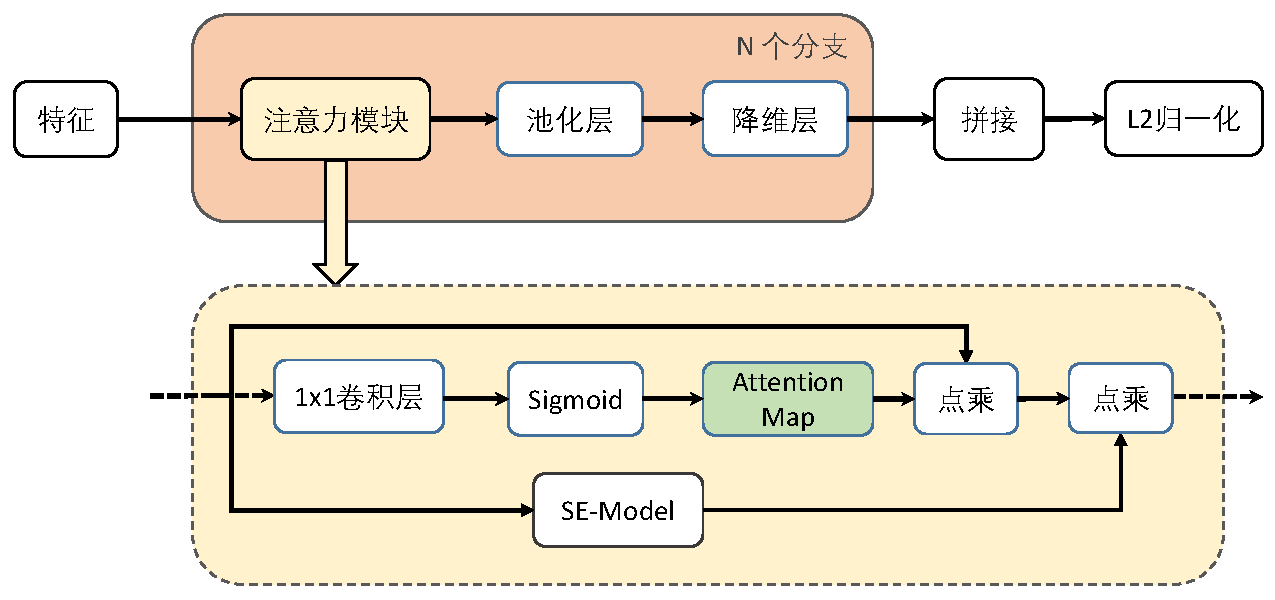
\includegraphics[width=1.0\linewidth]{Img/part.pdf}
  \caption{局部对齐网络的整体架构}
  \label{fig:partnet}
\end{figure}

\subsection{注意力模块}
本小节介绍如图\ref{fig:partnet}中所示的注意力模块。在局部对齐网络中,每一个分支都会生成一个掩膜$M_{i}$,这个掩膜的生成也是局部对齐的关键,其生成过程基于注意力机制,
我们称之为注意力模块。提出的注意力模块包括两个子模块:空间注意力模块和通道注意力模块。空间注意力模块学习空间维度的注意力分布;通道注意力模块则借鉴SE-Net的思想,
认为通道间具有互相依赖的关系,学习通道维度上的权重分布可以有效挖掘这种依赖关系以提升网络表达能力。这两个子模块有着相同的输入,即张量\textbf{T}。
\subsubsection{空间注意力}
对空间注意力的学习旨在挖掘对网络表达能力有益的局部区域特征,根据输入\textbf{T}学习得到一个二维的掩膜$M$并根据$M$更新输入\textbf{T},整个过程分为三个步骤:(1)
使用$1 \times 1$大小的卷积核做\textbf{T}做卷积操作,将\textbf{T}压缩为单通道的特征图。(2)对得到的单通道特征归一化处理,使得所有的特征值分布区间为0到1之间,归一化后
的特征称为注意力分布图(Attention map),即掩膜$M$。Attention map每个值的大小代表着学习到的注意力分布在这个区域的权重大小,特征值越大,注意力权重越大。
(3)将Attention map应用到的输入\textbf{T}之上,完成对空间局部信息的挖掘。

\begin{figure}[h]
  \centering
  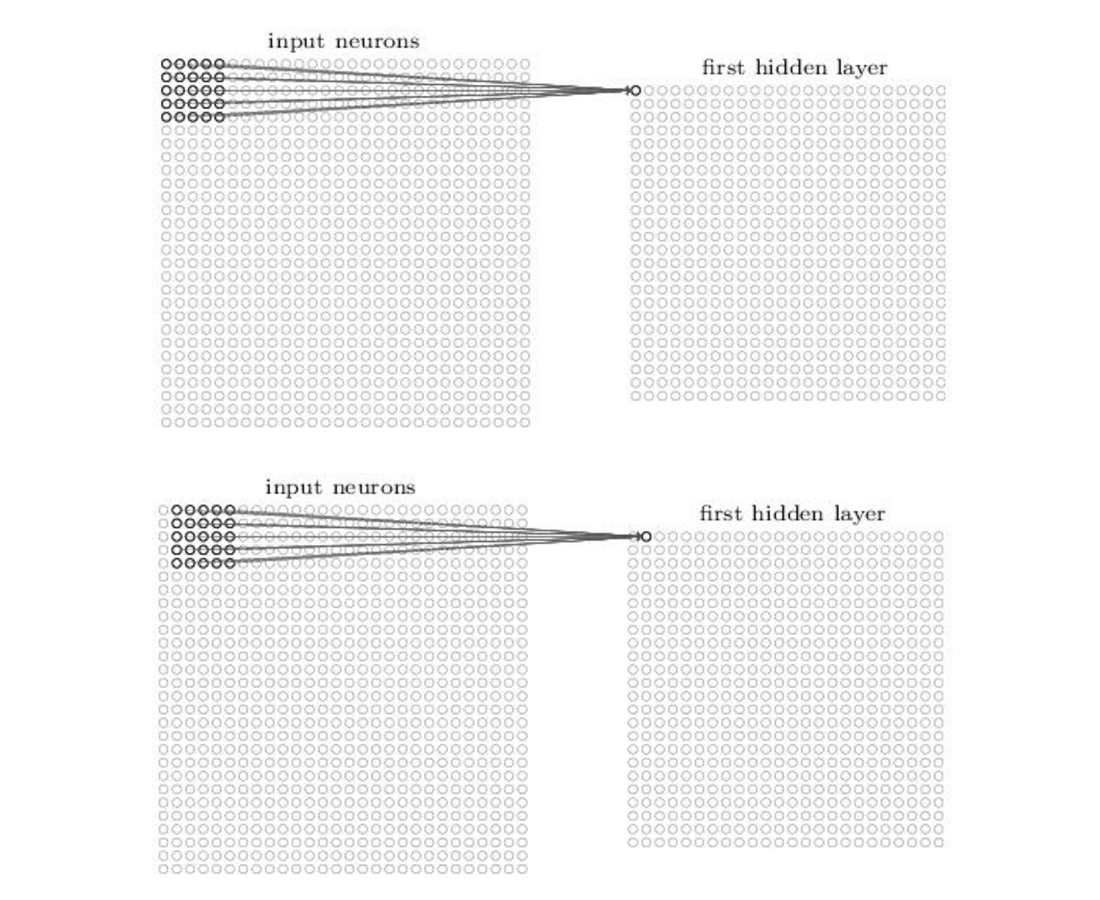
\includegraphics[width=1.0\linewidth]{Img/conv.pdf}
  \caption{对卷积操作的简要说明}
  \label{fig:conv}
\end{figure}

在卷积神经网络出现之前,深度神经网络的每一层网络都和全连接层相连接,下一层的每个输入节点都和当前层的所有输出节点相连接。对于计算机视觉来说,由于其输入是图像,
其空间位置信息对图像的语义理解有着非常重要意义,而全连接层由于和所有输入像素点连接,所以无法捕捉图像的空间信息,这样很不合理。卷积操作是卷积神经网络的核心,如图
\ref{fig:conv}所示,对于一个$28 \times 28$维度的输入,采用$5 \times 5$大小的巻积核通过滑窗的方式逐步计算输出值,这个$5 \times 5$的区域称之为感受野,每次只计算
感受野内部的特征且全局共享这个卷积核的参数,最后得到$24 \times 24$的输出。$5 \times 5$大小的巻积核包含25个权重参数$w$以及一个偏置参数$b$,每次滑窗的计算即卷积核所有权重和对应感受野特征值的相乘
后取和。本方法所提出的空间注意力模块第一步使用的卷积层采用$1 \times 1$大小的卷积核,这个做法的出发点基于$1 \times 1$卷积核的两个特性:(1)进行跨通道的特征交互与整合。
(2)对输入特征的维度变换。Attention map的生成应基于输入\textbf{T},且Attention map的空间维度应与\textbf{T}相同,即$w\times h$。
$1 \times 1$卷积层以\textbf{T}为输入,且与图\ref{fig:conv}中不同的是,卷积的输出可以保留特征的原空间大小,并将$c$个通道压缩至一个。

卷积层输出的特征图在维度上已经和我们需求的Attention map尺度一致,接下来需要对特征值做归一化,保证每个值的大小都在0至1之间,这里我们使用Sigmoid函数去实现归一化,
其表达式为:$\sigma(z)=\frac{1}{1+e^{-z}}$。
一般情况下,Sigmoid在深度神经网络中被用作激活函数,激活函数的意义在于引入非线性,而我们使用Sigmoid的原因在于它的一个重要特性:输出范围为0到1,
如图\ref{fig:sigmoid}所示。由于这个特性的原因,
Sigmoid除了作为激活函数外,也常常被用作二分类的概率输出层,其输出值表示类别为真的概率。在我们提出的注意力模块中,我们可以把Attention map的每个值看作一个二分类的
概率,表示当前区域是否是为需要分配更大权重的局部信息。
\begin{figure}[h]
  \centering
  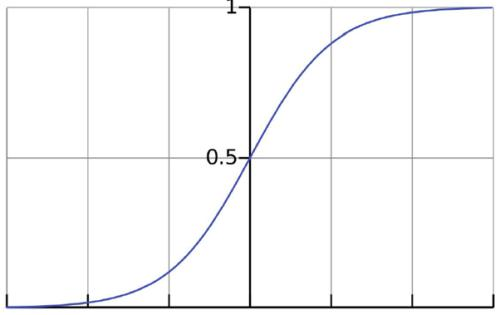
\includegraphics[width=10cm, height=6cm]{Img/sigmoid.jpg}
  \caption{Sigmoid函数}
  \label{fig:sigmoid}
\end{figure}


得到的Attention map为$w\times h$大小的二维特征图,而输入\textbf{T}的为$w\times h \times c$大小的张量,因此需要将Attention map复制$c$份,得到与\textbf{T}相同的尺寸,
两个张量做哈达马积(element-wise product)引入注意力权重,得到空间注意力模块的输出。

\subsubsection{通道注意力}
通道注意力模块借鉴自SE-Net,这个ImageNet 2017 竞赛图像分类的冠军架构在ImageNet 数据集上将 Top-5 error 降低到 2.251\%。近两年来,
SE-Net 因其强大的性能在深度学习领域被广泛使用,也为众多研究人员提供了新的思路和参考。由于SE-Net考虑的是特征图不同通道之间关联性,
所以其初衷并不是为了做视觉注意力,此处视觉注意力特指图像在空间维度的注意力。

Sun等人认为SE-Net通过调节通道间的权重分配也可以强化或者抑制特征图空间区域的局部响应强度,采用多个分支并行的方式,每个分支可以得到不同的局部高响应\cite{sun2018multi}。
这种同构多分支的网络设计方式本质是一种多特征融合,这种策略的有效性也已经在很多任务得到证明:
谷歌于2017年提出的Multi-head attention\cite{vaswani2017attention}将这种结构用于机器翻译任务,使得网络性能得到有效提升;
Hu等人将相同的理念应用在目标检测任务\cite{hu2018relation},也取得了成功。

通道注意力模块单分支的设计与SE-Net一致,如图\ref{fig:partnet}:首先通过全局平均池化(Global average pooling)将输入\textbf{T}压缩$c$维的向量,
然后经过全连接层(FC layer)编码学习通道注意力特征,最后经过Sigmoid归一化。得到的通道注意力向量与空间注意力模块的输出相乘后完成当前分支注意力模块的输出。

\subsection{跨域样本挖掘}
传统的机器学习方法要求源域数据和目标域数据具有相同的分布,从而保证在源域数据集训练的模型性能具有较高的可信度,然而在大多数情况下,训练网络模型的数据集和实际应用场景
之下的数据集很难具有同分布。因此,在已有源域数据训练出的模型的情况下,如何借助模型提取的特征知识,实现模型从源域到相似数据域的迁移具有重大的意义。
本节介绍一种结合在线三元组损失(Online triplet loss),通过已有模型在目标域挖掘无标签样本,并学习其数据分布,达到模型迁移的方法。

\subsubsection{网络训练}
\begin{figure}[h]
  \centering
  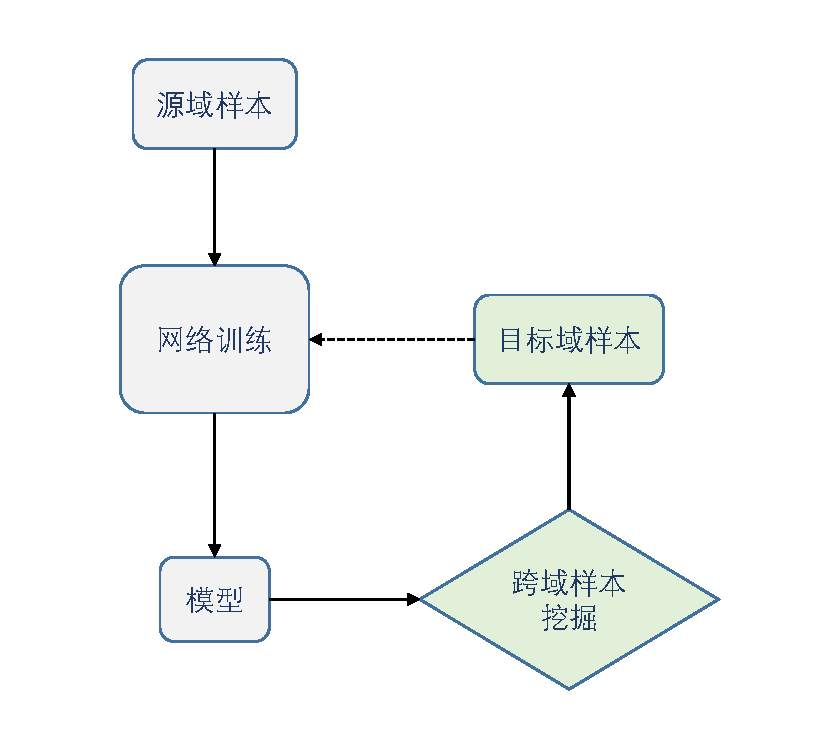
\includegraphics[height=10cm]{Img/crossdomain.pdf}
  \caption{网络训练流程图}
  \label{fig:crossdomain}
\end{figure}

本文所提出的跨域样本挖掘方法是一种可以复用,因此基于此方法的网络训练也是一种迭代的方式,如图\ref{fig:crossdomain}所示,网络的训练流程分为如下步骤:
\begin{itemize}
  \item[1.] 使用源数据域的数据组成训练集,并在此基础上训练出一个模型,训练用的深度网络采用上节所述的局部对齐网络。
  \item[2.] 根据步骤1训练所得模型在目标域做样本挖掘,这一过程会在目标域中获取一定量的样本,并附有标签信息。
  \item[3.] 将在目标域获取的样本和源域样本一起组成新的训练集,重新训练网络,得到新一轮的模型。
  \item[4.] 重复执行步骤2-3多次,直至模型性能稳定。
\end{itemize}

结合企业的实际应用场景来说,用于模型训练的数据一般来自商家拍摄的服装图像,这些数据也就是源域。而模型在实际使用时,输入是用户拍摄的服装图像,
这些由用户拍摄的图像数据集合可以看作是目标域。来自商家的样本一般拍摄质量较高,其中多数为模特摆排,光线等环境条件也比较稳定;而来自用户的检索样本随机性较强,
衣服的形状、摆放位置、光照条件、是否有遮挡或者旋转等因素都十分不稳定。因此,来自商家和来自用户的数据分布具有一定程度的区别。
此外,来自用户上传的检索图像没有标签信息,无法直接用于训练,采用人力标注的方式也不便执行,并且会耗费大量人力资源。

本节提出的跨域样本挖掘的方式可以在目标域挖掘无标签样本,并且可以为其生成伪标签用于网络训练。另外,用户上传的图像数据是一个不断增加的过程,随着目标域数据量的逐步递增
,其数据分布也是一个渐变的过程。基于跨域样本挖掘的网络迭代训练的模式则十分适合这个应用场景,在对过去所学习到的知识的基础上,不断迭代优化以适应新的数据分布,
本质上来说也是一种增量学习。
\subsubsection{样本挖掘}
\begin{figure}[h]
  \centering
  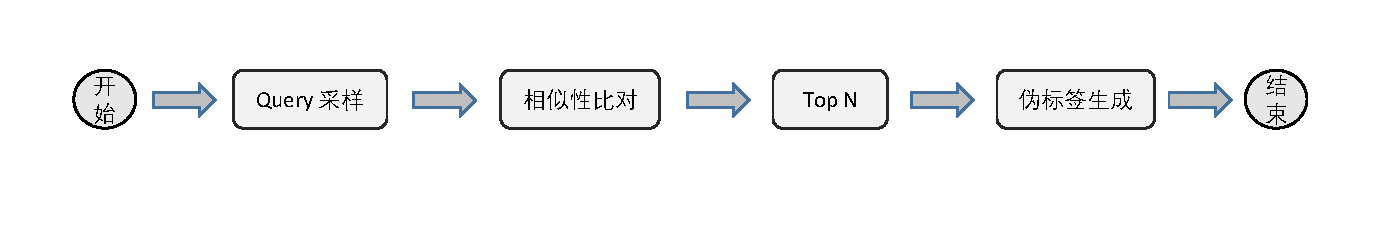
\includegraphics[width=1.0\linewidth]{Img/mining.pdf}
  \caption{样本挖掘流程图}
  \label{fig:mining}
\end{figure}

本小节详细介绍跨域样本挖掘的具体细节,挖掘流程如图\ref{fig:mining}所示:
\begin{itemize}
  \item[1.]Query 采样。我们把模型的输入,即待检索图像称为query,每次基于源域训练集训练得到一个模型之后,从目标域随机采样一部分图像query,剩下的图像作为检索库。
  \item[2.]相似度比对。检索任务的本质是基于相似度或者距离的排序任务,比对的对象是输入的query以及整个检索库里的所有样本。
  以步骤1得到的所有query作为模型的输入,在目标域做检索,根据检索库里图像特征和当前query对应的特征的相似度排序,我们保留top $N$的结果,即前N个和输入query最为相似的图像。
  \item[3.]伪标签生成。对与得到的top $N$的结果,认为前$m$个样本与query是同款服装,前$i$至$j$个样本与query是非同款样本,其中$0<m<i<j<N$。
\end{itemize}

挖掘到的样本对应的标签是上述算法得到的伪标签,伪标签最然没有绝对的准确性,但是是由模型的检索结果决定,所以按照伪标签去训练不会使模型的参数分布产生巨大变动。
\subsubsection{在线三元组损失}
如上文所述,训练时引入度量学习作为网络的监督,即Triplet loss。传统的三元组(triplet)组成采用离线的方式,在网络训练前将样本配成三元组,
训练时依次将所有的三元组送入网络。这种方法较为笨拙,预先组成的三元组数量非常庞大,用文本的方式保存也非常不灵活。我们采用在线组成三元组的方式训练网络,
有效简化了这一问题。
\begin{figure}[h]
  \centering
  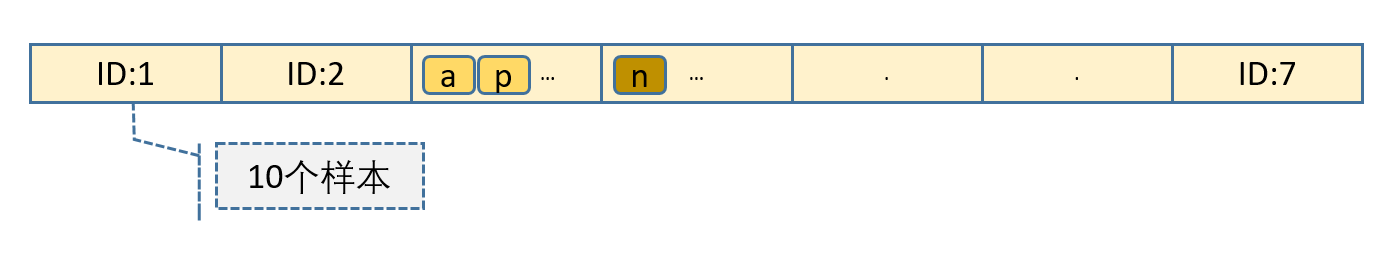
\includegraphics[width=1.0\linewidth]{Img/triplet.png}
  \caption{在线三元组的采样方式}
  \label{fig:triplet}
\end{figure}


在图\ref{fig:triplet}中描述了网络在训练过程中每个Batch的样本构成方式,Batchsize为70,共包含7个不同的ID,每个ID又由10个样本组成。由三元组的定义可知,任意两个来自相同
ID的样本,如图中的a(anchor)和p(positive),以及另一个来自任意不同ID的样本,如图中的n(negative)便可以组成一个三元组,网络在训练时在线遍历了当前Batch所有的三元组
并统计当前Batch所有三元组的损失的均值,每个ID的损失计算如公式\ref{eq:partnet:triplet}:
\begin{equation}
\label{eq:partnet:triplet}
\mathcal{L}_{ID}=\sum_{a=1}^{\left| ID \right|}\sum_{p=1}^{\left| ID \right|}\sum_{n=1}^{\bar{\left| ID \right|}} \{l(I_{a},I_{p},I_{n});p \ne a\}
\end{equation}
其中$\left| ID \right|$代表当前ID的样本总数,$\bar{\left| ID \right|}$代表除了当前ID外,Batch里其余所有样本的数量。

图\ref{fig:triplet}所描述的样本组成及损失计算方式适用于训练样本仅来自于源域的情况,当在源域的数据集下训练出第一个模型并在目标域挖掘出跨域的训练样本之后,后续网络训练
使用的在线三元组损失的计算策略作出了对应的调整。其中与图\ref{fig:triplet}描述的方式有如下几点区别:
\begin{itemize}
  \item[1.]训练样本来自两个域:源域和目标域。其中来自源域的训练样本包含M个ID;来自目标域的训练样本由跨域样本挖掘算法得到,包含N个ID,每个ID由挖掘算法中提及的query
    以及其检索对应的top $m$的样本组成。
  \item[2.]在每个Batch的组成过程中,随机从M+N个ID中采样,若采样得到的ID来自目标域的N个ID,则将这个ID的query对应的top $i$-top $j$组成第M+N个ID与之一起送入当前Batch,
    这种情况下的Batch构成与图\ref{fig:triplet-mining}一致,三种颜色分别代表了来自源域和目标域以及额外的ID:M+N。
  \item[3.]不统计属于ID:M+N的样本作为三元组里的a或者p时所产生的损失。其出发点也很容易理解:我们认为
    top $i$ - top $j$的样本含有大量噪声,应属于query的非同款样本,且他们本身不应看作同一款服装样本,但是当它们作为一个ID与top $m$对应的ID样本组成三元组时时可以使得
    top $m$的样本之间的距离越来越近,且top $m$的样本和top $i$ - top $j$之间的距离越来越远。
\end{itemize}
\begin{figure}[h]
  \centering
  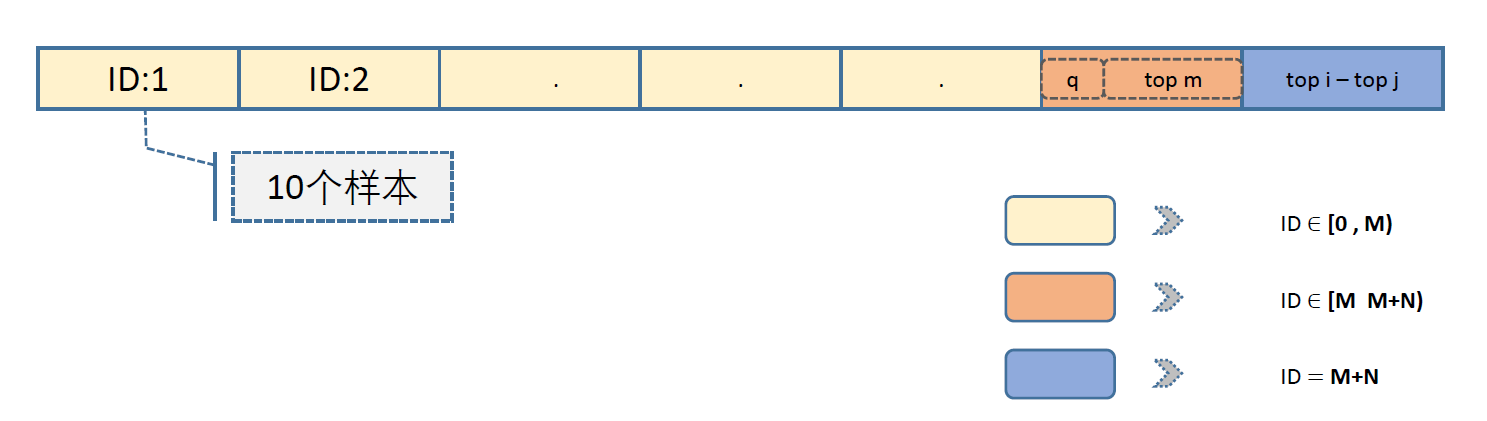
\includegraphics[width=1.0\linewidth]{Img/triplet-mining.png}
  \caption{包含跨域训练样本的Batch组成方式}
  \label{fig:triplet-mining}
\end{figure}


\section{实验与分析}
\subsection{数据集介绍}
全部实验在DeepFashion数据集上训练,DeepFashion是一个于2016年推出的大规模时尚服装数据库。整个数据集包含超过80万类的服装款式,覆盖了上装、下装、群装三大类服装,
其中的图像来源分为买家和卖家。来自卖家的图像拍摄质量较高,多数为在服装商店的摆拍;来自买家的图像则随机性较大,完全由消费者拍摄,没有摆放方式等规则限制。
数据集含有丰富的服装标注信息,除了款式标注之外还包括了检测框标注、关键点标注以及多种属性标注。检测框用于图像输入网络前的预处理;
属性信息一般指颜色、风格、尺寸、适宜人群等,在网络训练时常使用属性信息做监督以提高特征的语义表达能力。
\begin{figure}[h]
  \centering
  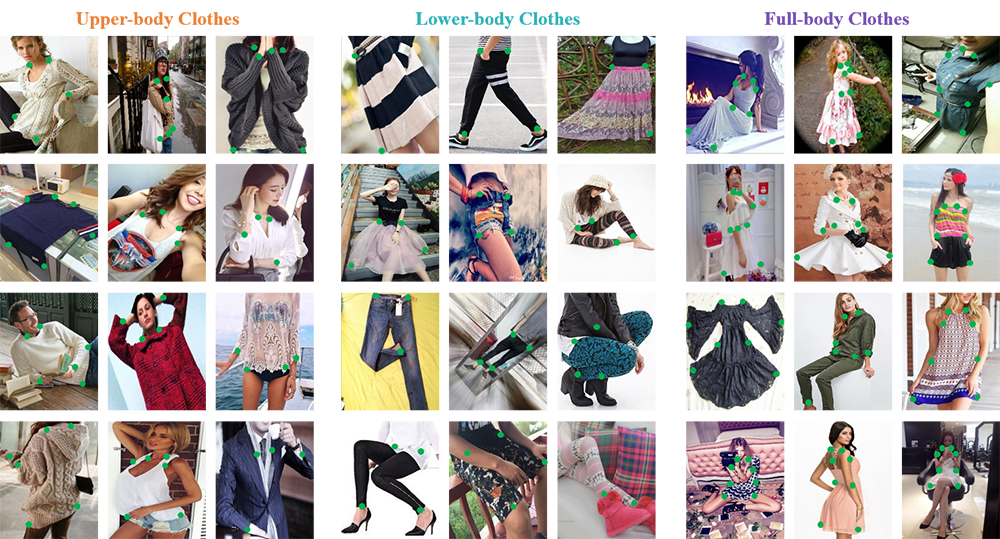
\includegraphics[width=0.9\linewidth]{Img/deepfashion.jpg}
  \caption{DeepFashion数据集\cite{liu2016deepfashion}}
  \label{fig:deepfashion}
\end{figure}


用于测试模型性能的测试集为阿里巴巴大规模图像搜索竞赛数据集(ALISC2015),这个数据集由三个部分组成:检索集(3,195,334张无标注图像)、验证集(1417张query,以及这些
query对应的同款服装图像及标注)、测试集(未公开,用于比赛提交时在线测试算法性能)。在ALISC2015数据集中,共包含十类图像类别:背包、饮料、家具、箱包、群装、上装、下装、饰品、零食、鞋子。
我们从验证集中挑出上装、下装以及群装三个类别,验证集中除了query以外的有标注的数据和检索集一起构成检索库,用于模型性能的测试,我们可以看出ALISC2015数据集的检索库中
带有标注的样本占着非常小的比例,可以较为准确的体现模型的性能。

\subsection{实验设置}
\subsubsection{评价指标}
模型检索性能的评价指标使用top 4的准确率,其定义为:检索返回的排序结果的top 4中至少出现一张同款服装图像的query数目所占所有测试query数目的比例。
\subsubsection{预处理}
由于ALISC2015中没有检测框的标注,我们使用方等人所标注的检测框\cite{fang2016object}。他们为ALISC2015中的每个类别标注了1000张图像,我们用这些标注图像训练Faster R-CNN,
使用AlexNet作为预训练模型。在对输入图像做检测时,每幅图最多输出一个检测框,若打分超出Faster R-CNN域值的检测框有多个,则取分数最高的那个。

我们基于目标检测预测的检测框对图像进行裁剪,对得到的图像较长的边缩放至统一尺寸(227个像素点),而较短的边按照与长边相同的缩放比例缩放,并在两侧Padding,
即填充值为零的像素点,这样所有的图像都可以统一为尺度$227 \times 227$的输入。
\begin{figure}[h]
  \centering
  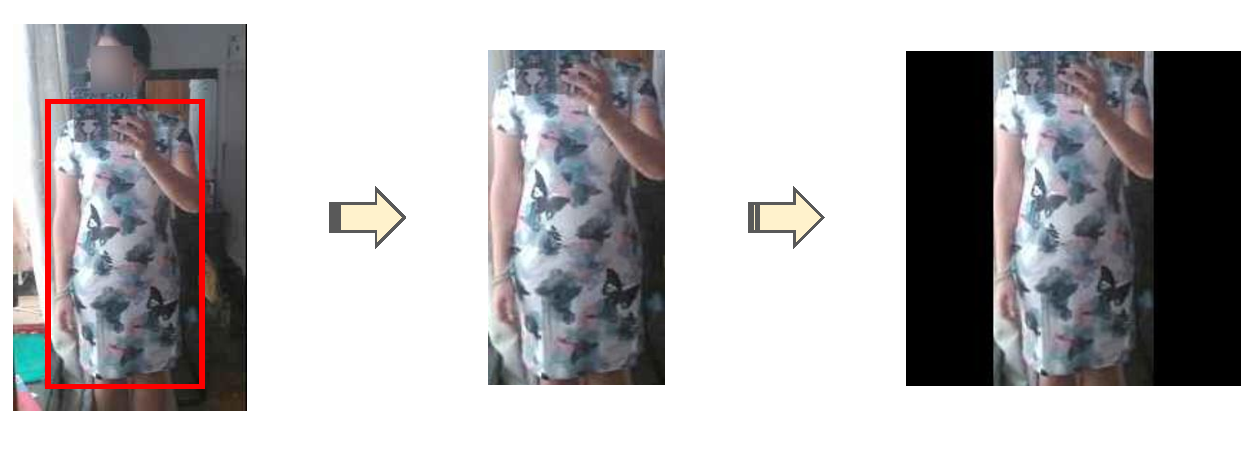
\includegraphics[width=0.8\linewidth]{Img/setup.pdf}
  \caption{对输入图像的预处理}
  \label{fig:setup}
\end{figure}

\subsubsection{数据增强}
对于电商平台使用基于图象内容的检索算法的实际应用场景来说,买家上传的检索图像(query)质量无法保障,常常会有旋转、遮挡、光线等的难以避免的因素使得模型的检索结果产生
一定的偏差。针对这些因素,我们在模型训练阶段对训练数据在以下几个方面做了数据增强,以提升模型的鲁棒性:
\begin{itemize}
  \item[1.]以一定概率对输入图像做水平翻转、竖直旋转(180旋转)以及随机小角度旋转。水平翻转可以使模型具有识别镜像中服装的泛化能力,因为有一部分买家拍摄的图像是对着
    镜子的自拍照;竖直旋转的数据增强是考虑到部分图像是买家将衣物摆放在床上拍摄,这种情况就会有上下颠倒的可能性;随机小角度的旋转是针对人体的姿势或者相机角度对
    拍摄图像角度产生的小幅度干扰。
  \item[2.]以一定概率对输入图像进行亮度和对比度的调整。光照因素对基于深度学习的计算机视觉任务一直都是十分重要的问题,不同的光线条件对模型性能的影响很大,如果只用
    室内的图像训练模型,那么模型对于室外的输入图像就很难识别。不同的服装图像可能拍摄于多种光照强度之下,因此对输入进行调整亮度、对比度的样本扩充很有必要。
  \item[3.]以一定概率对输入图像生成随机位置、随机大小的矩形掩膜,即将原始图像的某个矩形区域擦除,对应的像素值填充为0。Jon等人指出,这种随机的擦除策略
    对行人重识别算法的性能有明显的提升\cite{almazan2018re},其原因是对原图的随机的擦除类似于深度网络中常见的Dropout层,强制网络基于缺失部分信息的图像去学习,
    可以有效防止过拟合,提升网络泛化能力。在我们的实验中,掩膜的长和宽取在原图长和宽的$1/16$至$1/8$之间的随机数。
\end{itemize}
    
\subsubsection{特征提取网络}
实验使用SE-Inceptionv2作为特征提取网络,我们针对上装这一类对多个基础网络的基础性能(Baseline)做了对比,即用不同的基础网络训练分类任务,测试阶段取网络的Pool5层特征做检索测试,
实验结果显示SE-Inceptionv2的Baseline性能要高与其他的基础网络,如VGG、Inceptionv2、SE-ResNet152、ResNet152,SE-Inceptionv2指的是在Inceptionv2的网络架构中,
嵌入SE-Net的核心模块,这种结构得益与SE模块设计的灵巧性,SE-ResNet也是采用了同样的方式。具体实验结果如图\ref{fig:baseline}所示:
\begin{figure}[h]
  \centering
  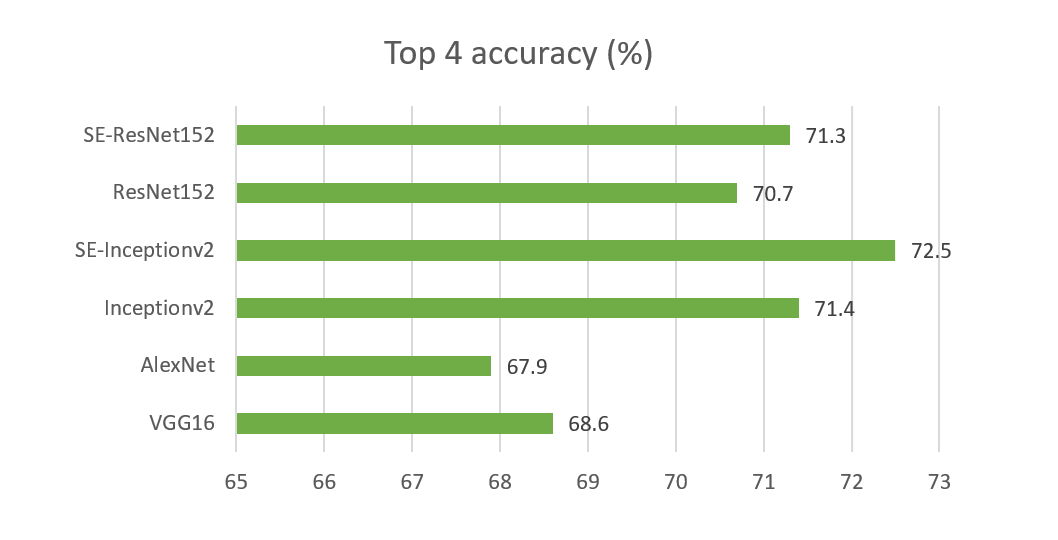
\includegraphics[width=0.8\linewidth]{Img/baseline.png}
  \caption{不同基础网络的Baseline性能对比}
  \label{fig:baseline}
\end{figure}


\subsubsection{损失函数}
本小节全面探究了度量学习与多任务学习对本方法性能产生的影响,使用SE-Inceptionv2作为特征提取网络,取Pool5的特征作为输入图像的最终表示。表\ref{tab:metric}中
ID loss指Softmax loss,用服装的类别信息监督;Attribute loss指使用DeepFashion中的属性标注作为辅助监督,每个类别的属性都对应一个多分类的任务,
比如颜色属性下对应多种具体的颜色类别。我们从实验结果可以得出以下结论:
% Table generated by Excel2LaTeX from sheet 'ablations'
\begin{table}[ht]
  \centering
  \caption{度量学习与多任务学习的有效性分析}
   \setlength{\tabcolsep}{6mm}{
    \begin{tabular}{l|ccc|c}
    \hline
    损失函数 & 上装 & 下装 & 群装 \\\hline
    \hline
    ID loss & 72.5  & 68.8  & 61.2  \\
		ID loss + Attribute loss& 73.0 &69.2& 62.3 \\
    Triplet loss & 74.4  & \textbf{71.0}  & \textbf{63.5}  \\
    Triplet loss + ID loss & \textbf{74.8}  &  70.5 & 63.2  \\  
    Triplet loss + ID loss + Attribute loss& \textbf{74.8}&70.3&63.2 \\
    \hline
    \end{tabular}%
    }
  \label{tab:metric}%
\end{table}%


\begin{itemize}
  \item[1.]实验表明在不引入Triplet loss时,Attribute loss作为辅助监督对网络性能有一定帮助。
  \item[2.]Triplet loss作用最为明显,相较于ID loss在每个服装类别都有两个点左右的提升,这充分证明了度量学习对于检索任务的有效性。
  \item[3.]在引入Triplet loss之后,ID loss和Attribute loss都不再能为网络的性能带来提升。
\end{itemize}
基于以上实验分析,本方法采用Triplet loss作为网络的损失函数,且不再使用额外的监督,如服装类别和属性信息等。
\subsection{注意力模块}
局部对齐网络的注意力模块包含空间注意力模块和通道注意力模块,如图\ref{fig:partnet},我们分别验证了这两个子模块的效果。
% Table generated by Excel2LaTeX from sheet 'ablations'
\begin{table}[ht]
  \centering
  \caption{空间注意力及通道注意力的有效性分析}
   \setlength{\tabcolsep}{6mm}{
    \begin{tabular}{l|ccc|c}
    \hline
    实验 & 上装 & 下装 & 群装 \\\hline
    \hline
    Baseline & 74.4  & 71.0  & 63.5  \\
    空间注意力 & 75.0  &  71.3 & 64.2  \\  
    通道注意力& 74.8 & 71.0 &63.9 \\
    空间注意力 + 通道注意力& \textbf{75.3}&\textbf{71.3}&\textbf{64.7} \\
    \hline
    \end{tabular}%
    }
  \label{tab:attention}%
\end{table}%


实验设置为单分支,即图\ref{fig:partnet}中的分支数K取1,表\ref{tab:attention}中,Baseline指的是表\ref{tab:metric}中第三组实验,即使用完整的SE-Inceptionv2网络。
使用空间注意力模块或者通道注意力模块替换SE-Inceptionv2最后一层卷积层之后的部分,网络性能均有提升,且结合空间与通道注意力的完整的注意力模块可以进一步提升性能,
这说明空间与通道的注意力学习可以互相促进。
\subsection{局部对齐网络}
本节探讨局部对齐网络分支数以及每个分支输出特征的维度对实验结果带来的影响。
\begin{figure}[h]
  \centering
  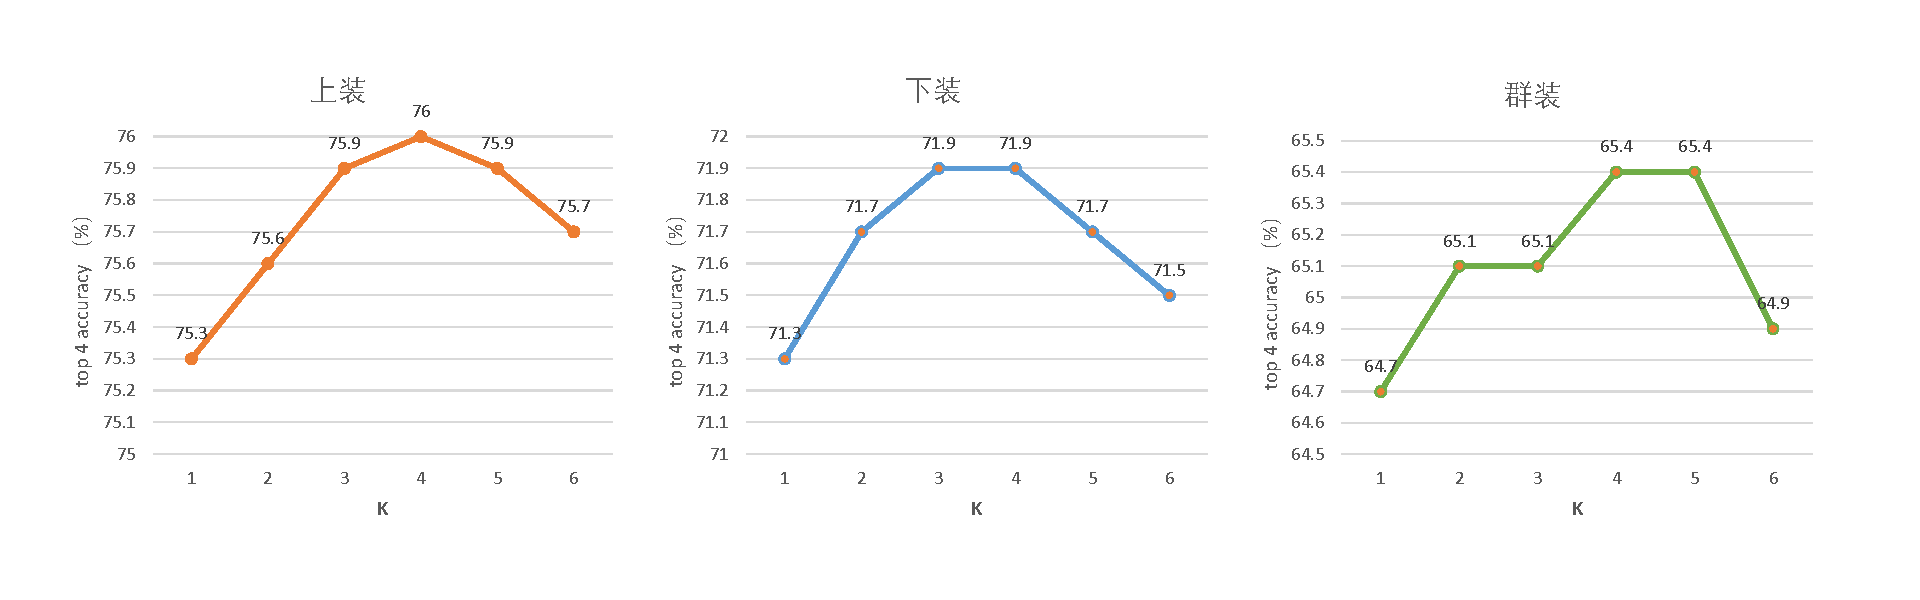
\includegraphics[width=1.0\linewidth]{Img/K.pdf}
  \caption{局部对齐网络分支数(K)对网络性能的影响}
  \label{fig:K}
\end{figure}

对于K值的对比实验如图\ref{fig:K}所示,K在取4时得到最好的实验结果,且K在取1到4时对应的性能呈现递增的趋势,K大于4时性能会逐渐下降。

所提出的局部对齐网络之所以设计为多个分支,是因为我们希望每个分支通过自己的注意力模块学习得到自己关注的局部区域,且不同的分支可以学得不同的注意力分布。
为了更直观的验证网络是否达到这个设计思路预期,对每个分支的Attetion map做了可视化分析。每个分支的Attention map均为$7 \times 7$大小,我们将Attention map
采用最近邻差值的方法上采样至原图大小($227 \times 227$),再将其复制为三份(RGB三个通道)并与原图做哈达马积,得到图\ref{fig:part-vis}的效果:
\begin{figure}[h]
  \centering
  \centerline{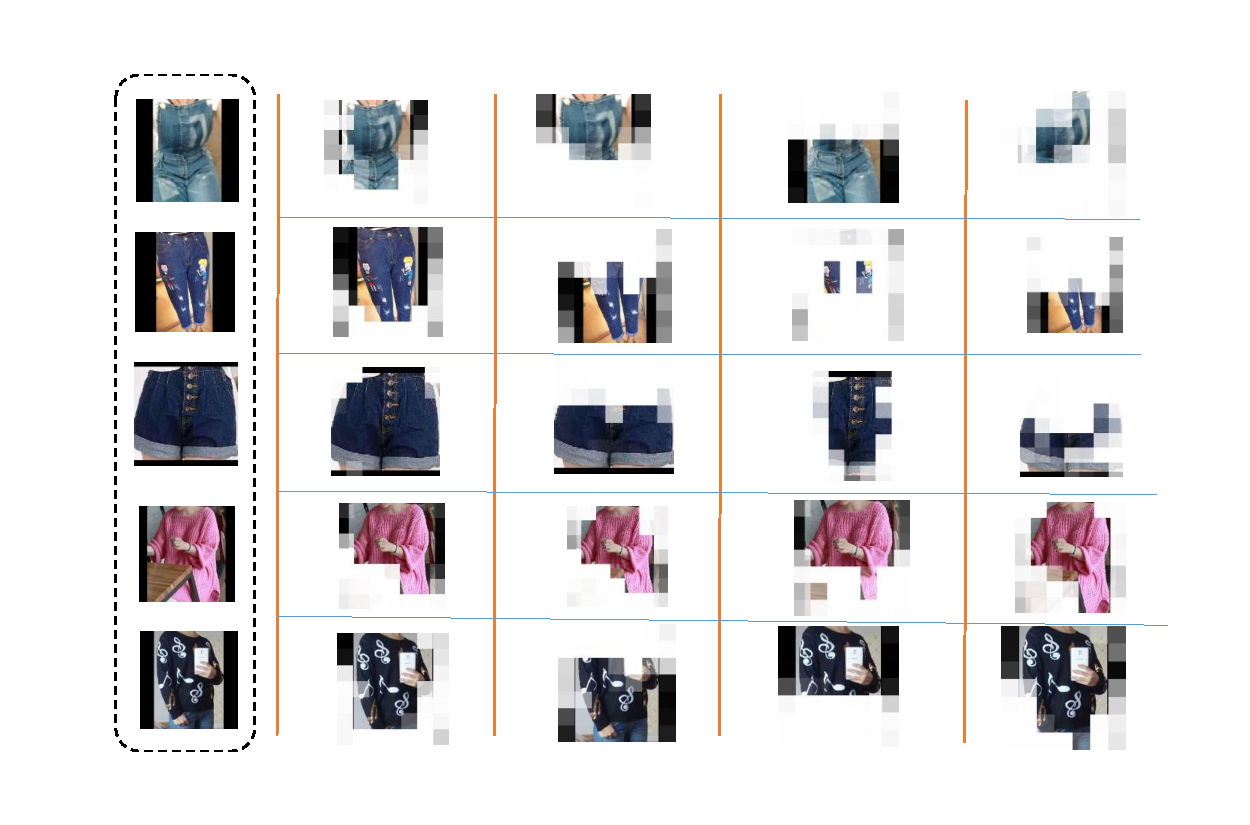
\includegraphics[width=1.2\linewidth]{Img/part-vis.pdf}}
  \caption{局部对齐网络不同分支Attention map的可视化}
  \label{fig:part-vis}
\end{figure}

其中第一列为输入网络的原图,右侧四列分别是局部对齐网络四个分支的注意力分布。我们可以看出即使网络的四个分支结构相同,但是其注意力分布却有所不同,有的分支注意力
偏向于服装的整体,仅仅抑制掉了图像的背景部分;有的分支注意力分布在服装的上半部分或者下半部分;还有的分支侧重于服装的细节部分,比如Logo图案等,
这种细节可能是区别这种款式服装与其他款式的关键信息。

% Table generated by Excel2LaTeX from sheet 'ablations'
\begin{table}[ht]
  \centering
  \caption{局部对齐网络单个分支特征维度对网络性能的影响}
   \setlength{\tabcolsep}{6mm}{
    \begin{tabular}{l|ccc|c}
    \hline
    单分支特征维度 & 上装 & 下装 & 群装 \\\hline
    \hline
    128 & 75.2&71.3&64.5 \\
    256 & 76.0&71.9&65.4 \\
    512 & 76.4&71.9&65.5 \\
    \hline
    \end{tabular}%
    }
  \label{tab:dim}%
\end{table}%


每个分支的输出维度由分支最后一层全连接层(图\ref{fig:partnet}中的降维层)维度决定,默认为256维,这也是由相关对比实验得出的结论。
单分支特征输出维度取256维时对比128维有较为明显的提升,而512维提升较为微弱,综合权衡检索算法消耗的时间与性能,降维至256维最为合适。
\subsection{跨域样本挖掘}
本小节讨论跨域样本挖掘算法的有效性,在所提出的样本挖掘算法中,由三个核心的参数,即决定目标域样本伪标签的$m$、$i$、$j$的取值。
由于这三个参数的组合总数量比较庞大,我们采取固定其中两个参数调节另一个的方式确定所调节参数的取值:首先令$i=30$,$j=40$,采用初始值为5,步长为5的方式调节$m$的取值,
根据不同的$m$、$i$、$j$的取值组合进行跨域样本的挖掘,并分别将从目标域挖掘得到的样本与来自源域的训练样本一起组成新的训练集进行下一轮的模型训练,对比模型的性能挑选出
最具优势的参数组合;确定下来$m$之后,$j$依然取40,用同样的方式,$i$在$m+5$至$j-5$之间调节,根据下一轮模型的性能确定$i$的取值。实验结果见图\ref{fig:mij},
\begin{figure}[h]
  \centering
  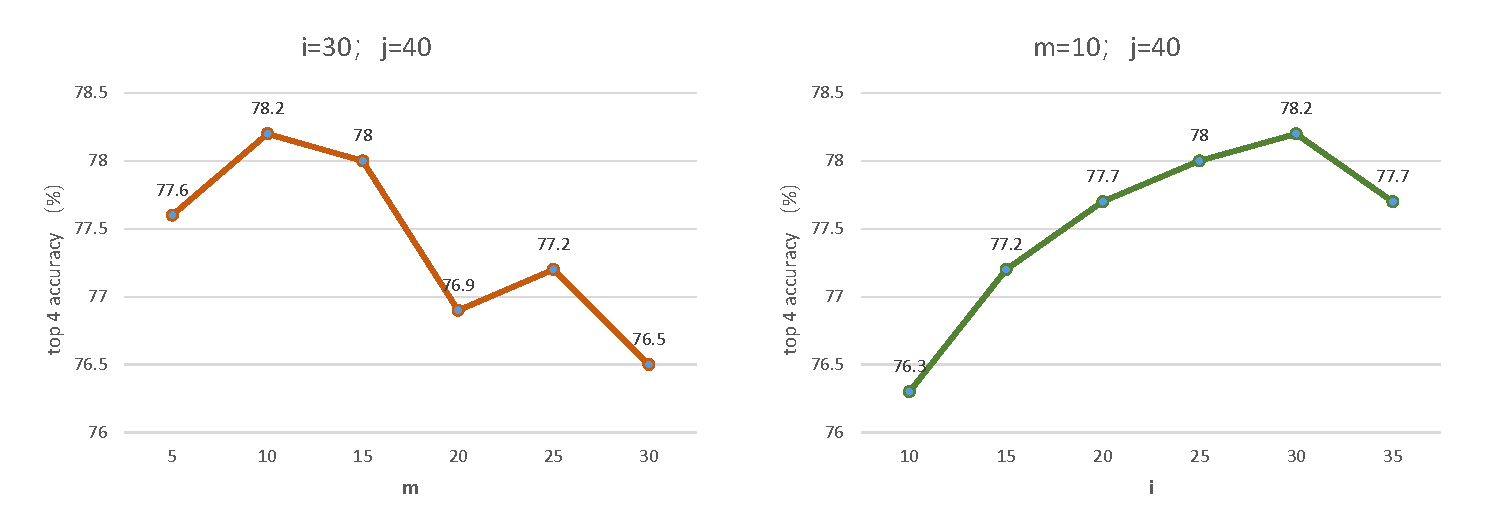
\includegraphics[width=1.0\linewidth]{Img/mij.pdf}
  \caption{伪标签生成相关参数(m、i、j)组合与第一轮挖掘后模型性能的对比试验}
  \label{fig:mij}
\end{figure}

由于上装、下装、群装三个类别的实验结果分布基本一致,图中只展示了上装的实验结果。
可以看出不同的伪标签生成区间性能有所区别,但相对于挖掘样本参与训练前的模型(只有源域数据参与训练的Baseline模型)的性能(76\%),
第一轮样本挖掘后训练的模型会有较为可观的提升。基于模型性能的分布,选择top 10的检索样本为query的同款,top 30至top 40的检索样本为query的非同款。
% Table generated by Excel2LaTeX from sheet 'ablations'
\begin{table}[h]
  \centering
  \caption{对基于跨域样本挖掘算法的网络训练不同迭代轮数的对比试验}
   \setlength{\tabcolsep}{6mm}{
    \begin{tabular}{l|ccc|c}
    \hline
    迭代次数 & 上装 & 下装 & 群装 \\\hline
    \hline
    0 & 76.0&71.9&65.4 \\
    1 & 78.2&72.7&66.5 \\
    2 & 79.8&74.1&67.8 \\
    3 & \textbf{80.2}&\textbf{74.8}&68.4 \\
    4 & 79.8&74.6&\textbf{68.7} \\
    \hline
    \end{tabular}%
    }
  \label{tab:mining-times}%
\end{table}%



本文所提出的基于跨域样本挖掘算法的网络训练流程是一个可迭代的过程,每次迭代得到的模型都可以重新用来做新一轮的样本挖掘,理论上来说迭代的次数并没有上限,
所以迭代停止的判断标准应是模型性能是否趋于稳定。我们将跨域样本挖掘一次并重新训练模型成为网络的一次迭代,网络的迭代次数与模型性能的变化如表\ref{tab:mining-times}所示:
迭代次数0作为Baseline,代表只由源域训练集训练的模型性能。网络迭代的前两次对模型性能提升都较为明显,这充分说明了所提出跨域样本挖掘算法的有效性。从第三次迭代以后,
模型的性能趋于稳定,这表明新的模型已经在一定程度匹配目标域的数据分布。
\section{本章小结}
本章提出了一种创新性的局部区域对齐网络,用于解决服装检索局部信息的定位与匹配问题。所提出的网络设计方式的核心方法基于注意力机制,这是一种借鉴自人类视觉信息处理方式
的机制,这种网络设计方式在训练时只需要服装样本的类别(款式)信息,不需要有关局部信息的任何标注去监督。与将服装图像切分为网格状或者条状不同,本章所提出的方法自适应
的定位输入图像的局部区域,这种对齐方式相对来说更为可靠和准确。

此外,基于在线三元组损失,本章还提出一种对跨域样本的挖掘算法。模型的跨域表现多数情况下都会有一定程度的下降,这是因为模型不能很好的匹配目标域的数据分布,所提出的
跨域样本挖掘算法基于源域训练的模型在目标域挖掘无标签样本,并给样本打上伪标签与源域训练集一起重新训练模型。算法可以迭代使用,通过挖掘目标域的无标签样本,使得模型
不断拟合目标域的数据分布,泛化能力也逐渐提升。这种迭代训练的方式类似于增量学习,可以很好的迎合企业的实际需求,随着用户上传的无标签数据的增加,可以每隔一段时间
实施一次样本挖掘保持模型的精度。
